
\chapter{商品检索与排序}

前文所述过程中建立的Lucene索引表和图像LSH哈希表是本章节商品检索与排序的根据,在本项目中,我们实现了两种检索方式——按关键词检索与按图片检索。

按关键词检索部分,用户可以输入商品关键词执行检索,也可以输入商品的品牌等属性执行高级检索。对检索的结果,用户可以选择按照相关度、价格顺序、评分高低进行排序。

在图片检索部分,用户上传图片后,可以选择LOGO匹配或精确匹配两种方式。\textbf{LOGO匹配}将图片与我们建立的产品品牌图库中的LOGO对比,计算SIFT特征向量的相似度,返回最有可能的品牌关键词执行关键词检索。\textbf{精确匹配}则将图片特征向量映射到前文建立的LSH哈希表中,返回匹配图片的URL列表,再到Lucene索引表中调用TermQuery匹配出URL对应的条目,按匹配度返回商品信息。

关键词检索与相关度排序沿用了本课程此前实验的代码,不作详述。本章节将主要介绍高级检索、商品排序和图片匹配三个功能的实现。

\section{商品高级检索}


\subsection{接口设计}

在此前建立索引的过程中,对于所有商品都具备的属性,如品牌、来源网站等,我们建立了专门的可被索引的Field进行存储,在本节我们将实现对这些Field的多字段检索。

在编写检索程序的代码前,考虑到我们的项目需要整合多种检索和排序方式,包括关键词、多字段检索、价格排序、评分排序等,我们有必要做好统一的接口,实现多重功能在后端查询时的一致。

一方面,用户可能在高级查询页面给出多字段的查询请求,对此我们采取了此前实验中类似的方法,编写了一个commandParser将查询条件转换成BooleanQuery处理多字段查询的请求。

尽管在查询首页中,用户输入的数据是以表单形式传入的,但我们在编写查询程序时,仍旧先将其转换成了一条“contents site:... brand:...”的字符串形式。之所以不直接提取表单内容而将其转换成字符串,是我们出于下文实现filter功能的考量,在filter功能中,用户在勾选过滤选项后会再次发出一个包含搜索的请求,网页需要保存记录此前搜索的字段传入filter请求的参数中,为了便于代码的复用,转换成字符串的方式会使程序更加可读和清晰。

另一方面,用户在结果页面可能会选择不同的检索方式,这会决定Lucene检索过程中searcher的参数,我们需要为此编写不同的搜索函数。在综合考虑整合以上两种因素后,以下是我们为检索程序提供的接口,可以看到,商品检索程序位于search\_command中,需要提供检索字符串kw和method(默认为按相关度relativity排序)两个参数。对获得的商品信息我们会做一些处理,获得filtertags等信息,具体将在前端部分进行介绍。

\begin{python}
# 统一处理搜索请求的web脚本 Web/code.py
class search:
    def GET(self):
        user_data = web.input(website="",brand="")
        kw = user_data.keyword
        if user_data.brand:
            kw += ' brand:%s' %(user_data.brand)
        if user_data.website:
            kw += ' website:%s' %(user_data.website)   # 将输入表单转换成字符串形式的请求
        method = web.input(method="relativity").method.decode('utf-8')
        vm_env.attachCurrentThread()
        contents = search_command(kw,method)     # 搜索结果
        filtertags = total(contents)           # 统计品牌、属性、特色的结果,即显示在页面左侧所必须的内容
        results = itemlis(contents)            # 要显示在页面右侧的所必需的内容
        return render.result(kw,method, results, filtertags)
\end{python}

\subsection{多字段查询处理}

在检索程序中,我们首先要对输入的query字符串进行处理,为此我们编写了一个command\_to\_query函数,统一处理各种形式的query。

\begin{python}
def command_to_query(command,analyzer):
    command_dict = parseCommand(command)          # 将字符串query转换成dict形式
    print command_dict
    seg_list = jieba.cut(command_dict['title'])
    command_dict['title'] = (" ".join(seg_list))  # 对command_dict遍历,建立BooleanQuery
    querys = BooleanQuery()
    for k,v in command_dict.iteritems():
        query = QueryParser(Version.LUCENE_CURRENT, k,
                            analyzer).parse(v)
        querys.add(query, BooleanClause.Occur.MUST)  # 各字段之间为AND关系
    return querys
\end{python}

对不同的检索方式,我们设计了如下结构以调用不同的搜索函数。
\begin{python}
def search_command(query,method):
    ... # 配置searcher、analyzer
    return globals()[method+'_search'](searcher,analyzer,query)
    # 根据method的不同调用不同函数名的搜索函数
\end{python}

至此,我们完成了搜索程序接口的设计,并且实现了商品的多字段高级搜索。

\section{商品按属性排序}

对具体的函数设计而言,我们有按相关度排序、按价格排序和按评分排序。相关度排序检测搜索结果与商品名称信息的匹配度,可以调用Lucene内置的scoreDocs方法实现,在此前的实验中已经完成,不作详述。对价格和评分排序,我们在建立索引时已经将这些信息用Lucene内置的LONG Field进行存储,我们只需为其建立对应的SortField,Lucene就可以实现按排序执行查找,以按评分查找为例,对应搜索程序的脚本如下所示。

\begin{python}
def rank_search(searcher, analyzer, command):
    rank_sorter = Sort(SortField("score",SortField.Type.LONG,True))  # True表明降序排序
    query = command_to_query(command,analyzer)
    scoreDocs = searcher.search(query, 150, rank_sorter).scoreDocs
    return read_results(scoreDocs,searcher) 
    # read_results函数提取搜索结果中的必要信息,将在前端部分介绍
\end{python}

\section{按图片检索}

\subsection{图片匹配}
根据我们已经建立的Hash表中包含了网页的URL和直方图特征向量。执行查询时,对输入的图片文件,我们计算图片文件的特征向量,将特征向量通过建表时相同的哈希函数映射到5张哈希表中,由LSH的局部敏感性质,我们认为哈希映射击中单元中的所有元素都和查询query具有一定的相似性。取5张哈希表中击中单元的并集,计算待查询的特征向量与我们存储的特征向量的相似度,就可以按序给出最接近的若干URL。

在查询的过程中,我们仅计算了5个哈希值,并仅对取出的n个元素(n远远小于数据集规模N)计算了匹配度,因此所消耗的时间是与数据集无关的常数时间。此外,由于我们的特征向量已经存放在了哈希表中,因此也可以保证计算匹配度的时间相较数据集规模N是常数的。该查询方式能够在时间上达到理想的效率。

\begin{python}
# 匹配图片函数
def match_pict(img):
    docs = []
    imgfeat = get_feature_Local(img)             # 计算查询图片的特征向量
    with open("hash_table.json",'r') as load_f:  # 打开本地哈希表文件
        load_list = json.load(load_f)
        for j in range(0,5):
            hash_val = LSHash(img,proj[j])       # 对查询图片进行哈希映射
            hits = load_list[int(hash_val)]      # 取出映射结果
            for hit in hits:
                elem = hit[0],similarity(imgfeat,hit[1])
                if elem not in hit:
                    hit.append(elem)             # 加入待排序集
    docs_sorted = sorted(docs,key = lambda kv:(kv[1]))
    res_lis = [i for (i,j) in docs_sorted[:50]]  # 取前50匹配的结果
    return res_lis                               # 返回50个最匹配的URL条目
\end{python}

\subsection{匹配条目查询}

上述过程中返回了一个URL列表,注意到URL是区分不同商品信息的标准,因此理论上有了URL就可以将搜索结果呈现在网页中。但不同于其他查询方式中返回包含所有信息的索引文档列表,在这里我们还需要对哈希表返回的URL列表元素在Lucene索引库中再查询,以获得商品的完整信息呈现在网页上,我们采用TermQuery的方式进行查询,如下所示。

\begin{python}
def pict_search(img):
    urls = match_pict(img)             # 调用上文match_pict函数执行LSH查询
    ... # 配置searcher,analyzer
    res_lis = []
    for url in urls:
        query = TermQuery(Term("url",url))   # 调用Lucene的TermQuery查询
        scoreDocs = searcher.search(query, 1).scoreDocs
        res_lis += read_results(scoreDocs,searcher)
    return res_lis                     # 返回的格式与其它查询函数接口一致
\end{python}


\part{Web Front-end}

\chapter{Web框架}

在本项目中,前端的搭建基于web.py框架,在页面美化方面采用了Bootstrap框架。下面对Web前端的工作作具体介绍。

\section{web.py配置}

网站前端的URL结构如图\ref{fig:zlt_url}所示。

\begin{figure}[htbp]
\centering
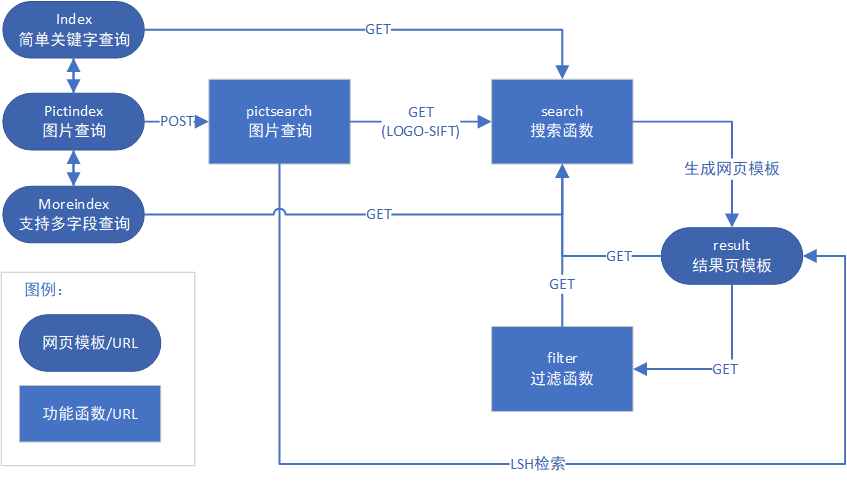
\includegraphics[width=13.5cm]{img/zlt/url.png}
\caption{网页URL组织形式}
\label{fig:zlt_url}
\end{figure}

在首页中,用户可以选择三种不同的搜索方式,对应三种表单,分别发起不同的request。简单的关键词搜索和支持多字段的高级检索会发起GET请求,将检索query传入上文构建的search函数。

上传图片的操作则会发起POST请求,POST请求首先将用户上传的文件保存到服务端,再根据用户选择的查询方式(LOGO匹配或精确匹配),调用对应的函数,返回响应的结果,处理POST请求的脚本如下所示。

\begin{python}
class pictsearch:
    def POST(self):
        x = web.input(input_img={})
        filedir = 'static/userupload'
        if 'input_img' in x:  # to check if the file-object is created
            fout = open(filedir + '/' + 'tmp', 'wb')
            # creates the file where the uploaded file should be stored
            fout.write(x.input_img.file.read())
            # writes the uploaded file to the newly created file.
            fout.close()  # closes the file, upload complete.
        # 将文件保存到本地
        if web.input().method == 'logo':
            kw = logo_recognition("static/userupload/tmp")  
            # 调用SIFT匹配函数,返回匹配的品牌关键词
            vm_env.attachCurrentThread()
            contents = search_command(kw,'rank'.decode('utf-8'))
            filtertags = total(contents)
            results = itemlis(contents)
            return render.result(kw, 'rank', results, filtertags)
        else:
            vm_env.attachCurrentThread()
            contents = pict_search("static/userupload/tmp")
            # 调用LSH检索函数,返回匹配列表
            filtertags = total(contents)
            results = itemlis(contents)
            return render.result('LSH Match', 'rank', results, filtertags)
\end{python}


无论是针对关键词还是图片的search函数,返回值均为一个包含所有检索匹配文档的列表,该列表会作为构造结果页模板的主要参数,决定结果页中的内容。结果页中也包含一个搜索表单和过滤选项,因此也可以发起搜索或过滤的GET请求,再次调用search或filter函数,刷新结果页的内容。

\section{网页功能的实现}

\subsection{搜索主页}

搜索主页如图\ref{fig:zlt_index1}、\ref{fig:zlt_index2}、\ref{fig:zlt_index3}所示


\begin{figure}[htbp]
\centering
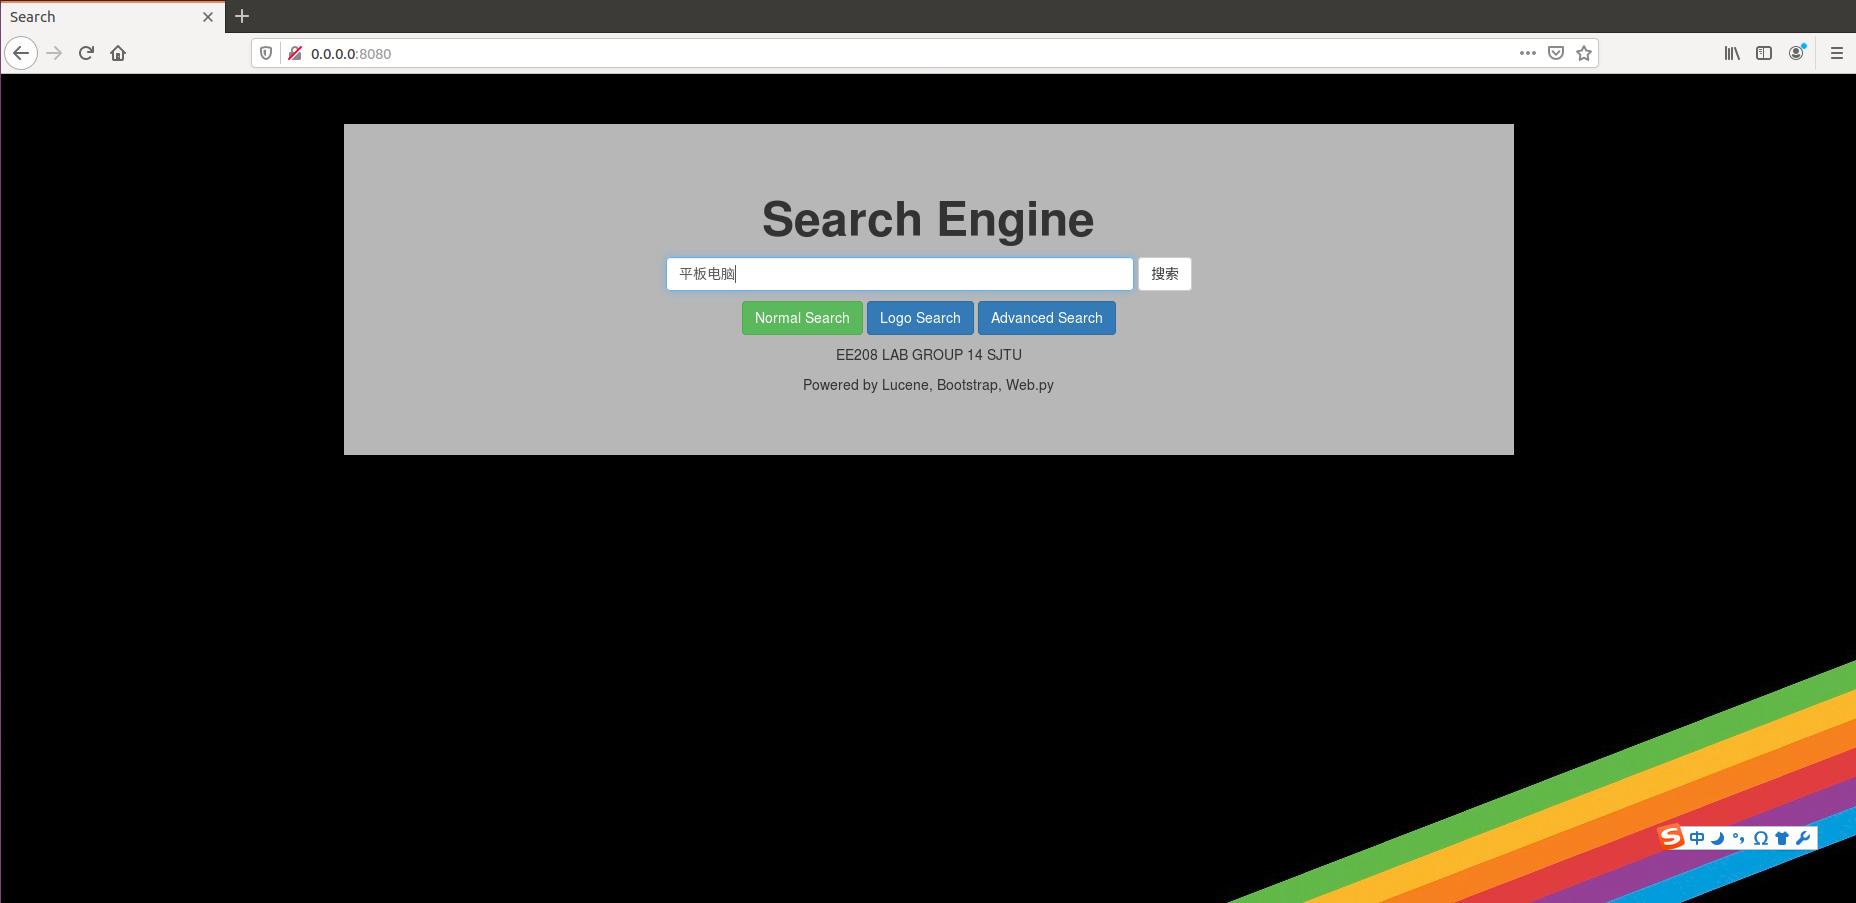
\includegraphics[width=13.5cm]{img/zlt/searchidx1.png}
\caption{单关键词查询首页}
\label{fig:zlt_index1}
\end{figure}

\begin{figure}[htbp]
\centering
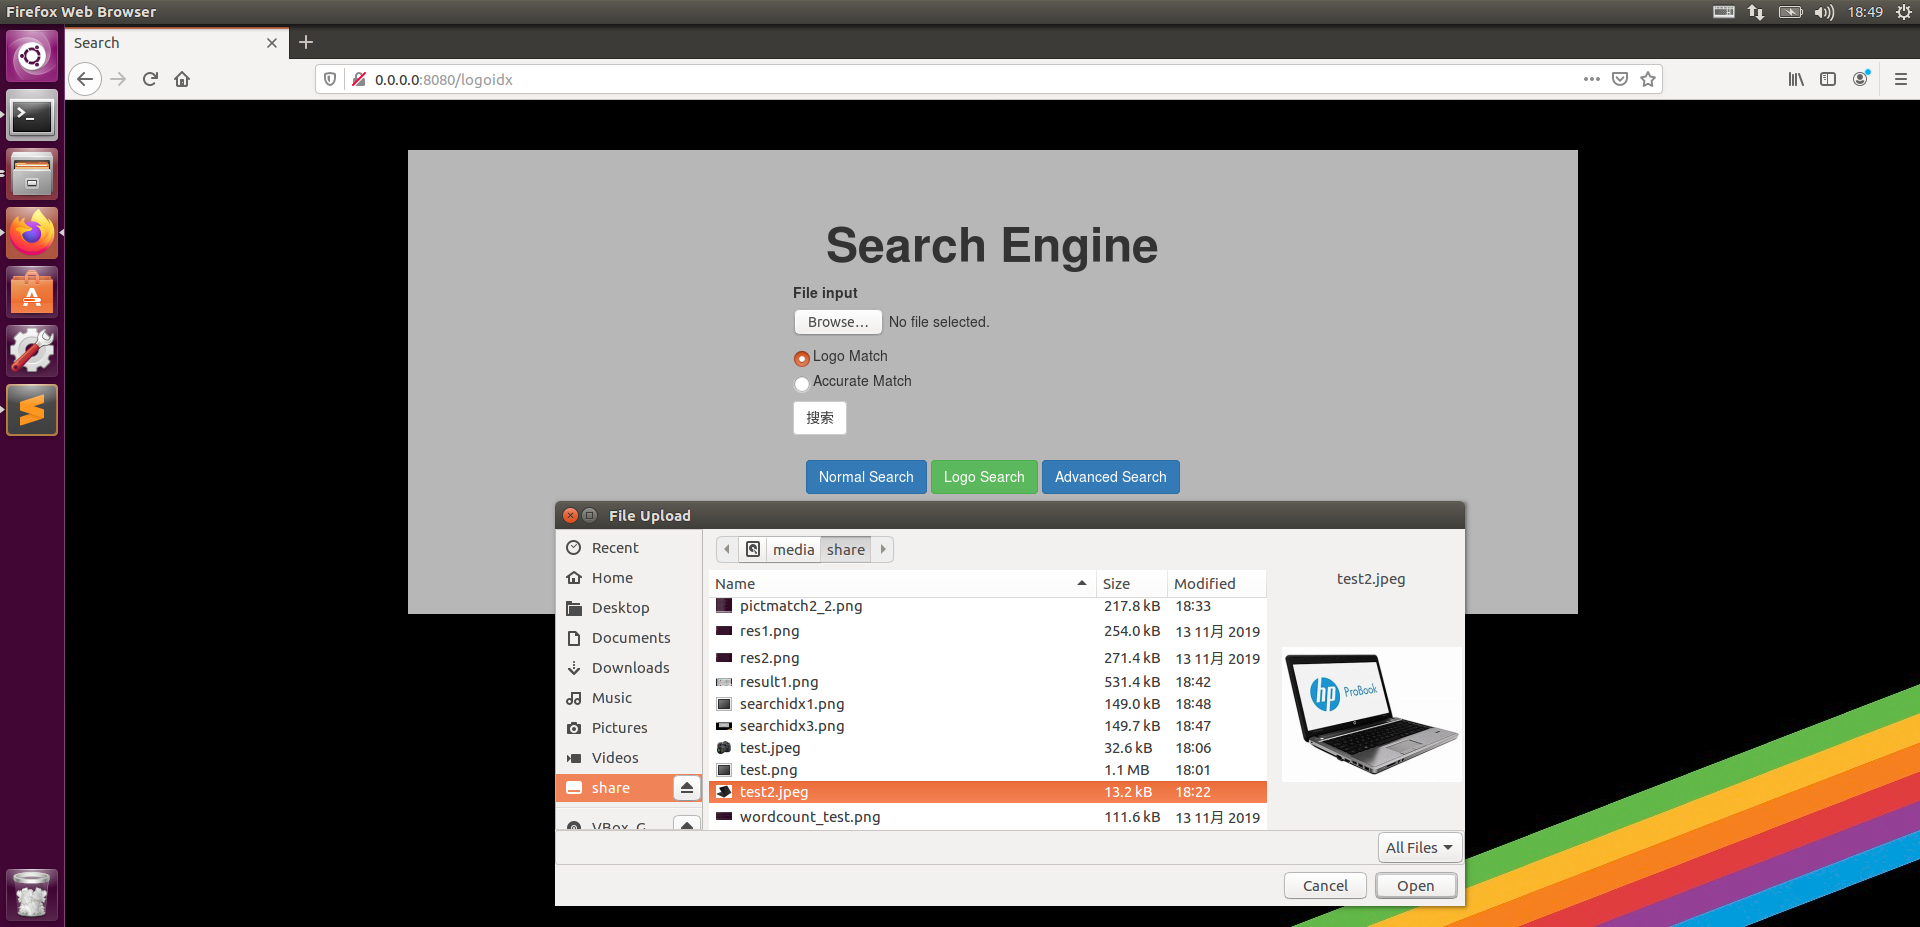
\includegraphics[width=13.5cm]{img/zlt/searchidx2.png}
\caption{图片查询首页}
\label{fig:zlt_index2}
\end{figure}

\begin{figure}[htbp]
\centering
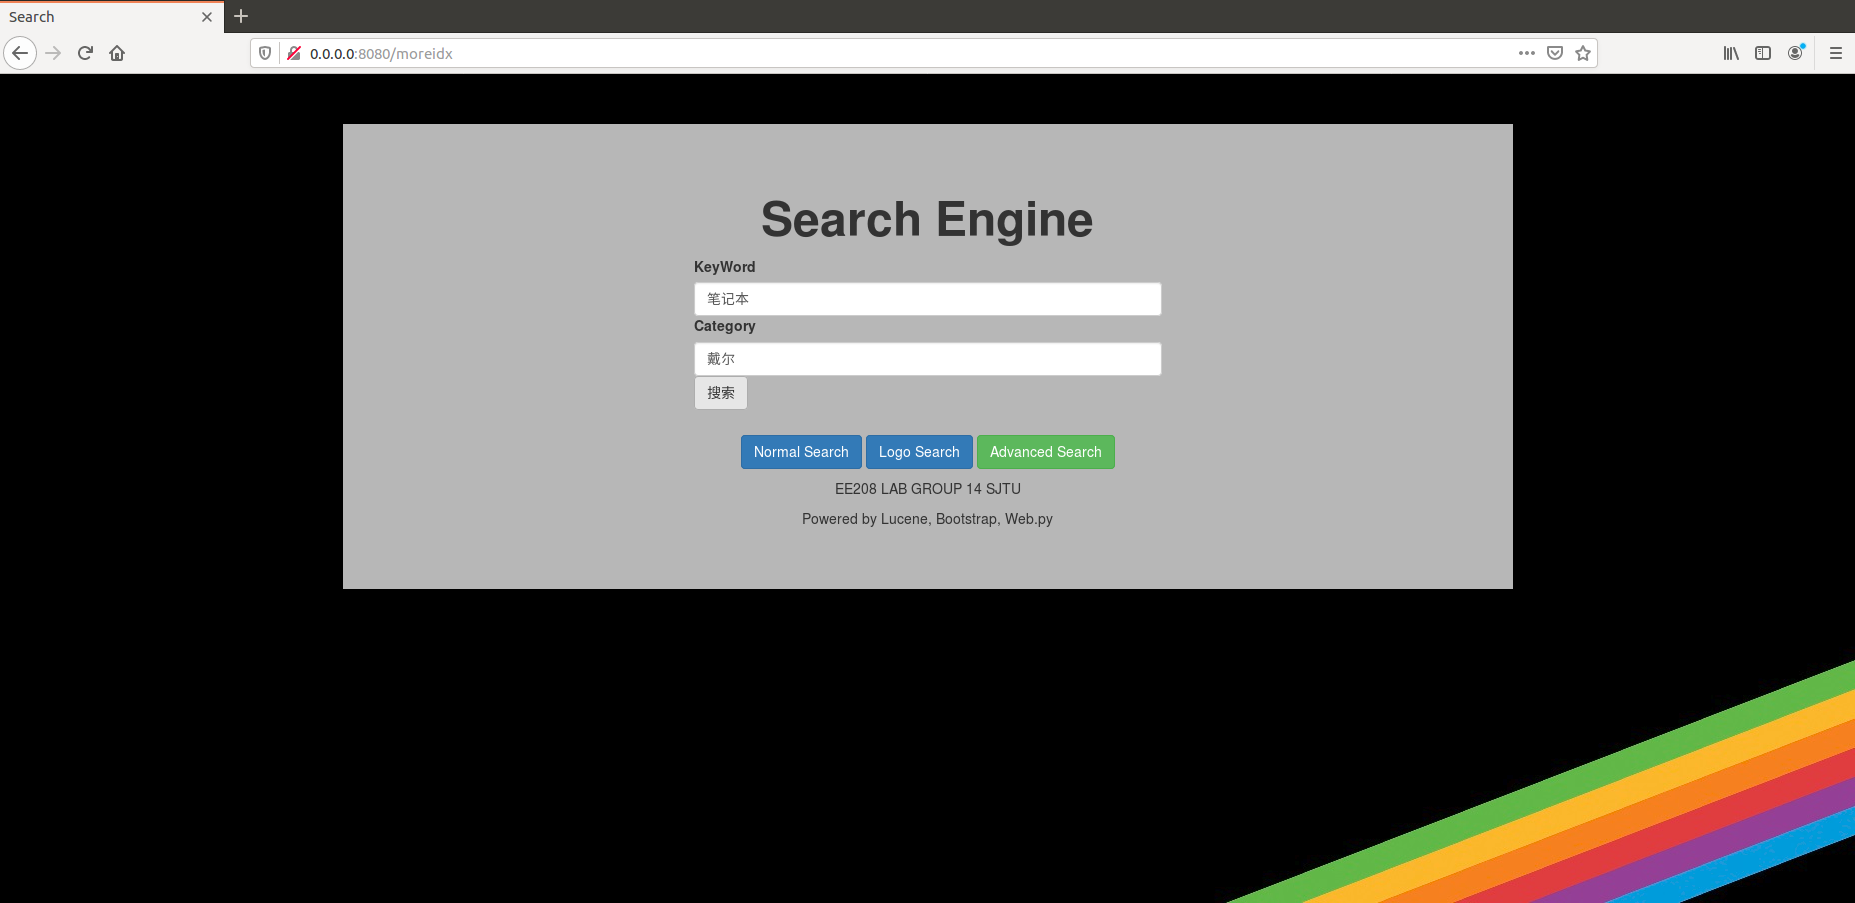
\includegraphics[width=13.5cm]{img/zlt/searchidx3.png}
\caption{多字段查询首页}
\label{fig:zlt_index3}
\end{figure}

\subsection{商品信息陈列}

\subsection{商品过滤功能}

\section{网页美化}

\subsection{Bootstrap框架}




\chapter{项目成果}